\documentclass[10pt, a4paper]{article}

% ============================================================================
% PACKAGES & PAGE GEOMETRY (Calibrated for a strict 2-Page Main Report Body)
% ============================================================================
\usepackage[utf8]{inputenc}
\usepackage[T1]{fontenc}
\usepackage{newtxtext, newtxmath} % Formal Times-style academic font
\usepackage[a4paper, top=1.55cm, bottom=1.55cm, left=1.7cm, right=1.7cm]{geometry}
\usepackage{graphicx}
\usepackage{booktabs}
\usepackage{array}
\usepackage{xcolor}
\usepackage{listings}
\usepackage{enumitem}
\usepackage{titlesec}
\usepackage{fancyhdr}
\usepackage{caption}
\usepackage{subcaption}
\usepackage{tikz}
\usepackage{datetime2}
\usetikzlibrary{shapes.geometric, arrows.meta, positioning}
\usepackage{xurl} % Ensures long bibliography URLs wrap cleanly without margin overflow
\usepackage[colorlinks=true, linkcolor=blue!60!black, citecolor=blue!60!black, urlcolor=blue!60!black]{hyperref}


\definecolor{codebg}{RGB}{246, 248, 250}
\definecolor{codeframe}{RGB}{208, 215, 222}
\definecolor{codegreen}{RGB}{40, 120, 60}

% ============================================================================
% COMPACT ACADEMIC SPACING FOR STRICT 2-PAGE LIMIT
% ============================================================================
\setlength{\parindent}{0pt}
\setlength{\parskip}{2.5pt}
\setlist[itemize]{noitemsep, topsep=1pt, leftmargin=1.4em}
\setlist[enumerate]{noitemsep, topsep=1pt, leftmargin=1.5em}

\titleformat{\section}
  {\normalfont\large\bfseries}{\thesection.}{0.5em}{}
  [\vspace{0.5pt}]
\titlespacing*{\section}{0pt}{5pt}{2.5pt}

\titleformat{\subsection}
  {\normalfont\normalsize\bfseries}{\thesubsection}{0.5em}{}
\titlespacing*{\subsection}{0pt}{3.5pt}{1.5pt}

% Compact Bibliography Formatting so all 4 References fit cleanly on Page 2
\renewcommand{\refname}{Bibliography}
\makeatletter
\renewenvironment{thebibliography}[1]
     {\section*{\refname}%
      \scriptsize
      \list{\@biblabel{\@arabic\c@enumiv}}%
           {\settowidth\labelwidth{\@biblabel{#1}}%
            \leftmargin\labelwidth
            \advance\leftmargin\labelsep
            \setlength{\itemsep}{1.5pt}%
            \setlength{\parskip}{0pt}%
            \setlength{\parsep}{0pt}%
            \@openbib@code
            \usecounter{enumiv}%
            \let\p@enumiv\@empty
            \renewcommand\theenumiv{\@arabic\c@enumiv}}%
      \sloppy
      \clubpenalty4000
      \@clubpenalty \clubpenalty
      \widowpenalty4000%
      \sfcode`\.\@m}
     {\def\@noitemerr
       {\@latex@warning{Empty `thebibliography' environment}}%
      \endlist}
\makeatother

% ============================================================================
% HEADER & FOOTER CONFIGURATION
% ============================================================================
\pagestyle{fancy}
\fancyhf{}
\fancyhead[L]{\footnotesize\textit{ENG2083: Introductory Programming 2 -- Final Assignment (Lab 8, Option 6)}}
\fancyhead[R]{\footnotesize\textit{2962389m}}
\fancyfoot[C]{\footnotesize Page \thepage}
\renewcommand{\headrulewidth}{0.4pt}

% ============================================================================
% CODE SNIPPET STYLING (For the single 3-line excerpt on Lines 178-180)
% ============================================================================
\lstdefinestyle{pythonstyle}{
    language=Python,
    backgroundcolor=\color{codebg},
    frame=single,
    rulecolor=\color{codeframe},
    basicstyle=\ttfamily\footnotesize,
    keywordstyle=\bfseries\color{blue},
    stringstyle=\color{codegreen},
    commentstyle=\itshape\color{gray},
    numbers=left,
    firstnumber=178,
    numberstyle=\tiny\ttfamily\color{gray},
    numbersep=6pt,
    aboveskip=2.5pt,
    belowskip=2.5pt,
    showstringspaces=false,
    tabsize=4
}

% ============================================================================
% SAFE IMAGE MACRO (Compiles cleanly even before you upload images!)
% ============================================================================
\newcommand{\safeimage}[3][0.5\textwidth]{%
    \IfFileExists{#2}{%
        \includegraphics[width=#1]{#2}%
    }{%
        \fcolorbox{blue!60}{gray!8}{%
            \parbox[c][4.2cm][c]{#1}{%
                \centering\color{blue}\bfseries #3\\[4pt]
                \footnotesize\normalfont\color{black!70}
                (Upload \texttt{#2} to Overleaf project tree to render image)
            }%
        }%
    }%
}

\begin{document}

% ============================================================================
% TITLE PAGE (Does not count toward the 2-page report limit)
% ============================================================================
\begin{titlepage}
    \centering
    \vspace*{1.0cm}
    
    % University of Glasgow Logo Placeholder / Image
    \IfFileExists{uofg_logo.jpg}{%
        
\includegraphics[width=0.52\textwidth]{uofg_logo.jpg}
    }{%
        \fcolorbox{blue}{white}{%
            \parbox[c][3.0cm][c]{0.65\textwidth}{%
                \centering
                {\Large\bfseries\color{black} UNIVERSITY OF GLASGOW}\\[4pt]
                {\normalsize\scshape School of Engineering}\\[6pt]
                {\footnotesize\color{gray} [Upload \texttt{uofg\_logo.png} to Overleaf to display official logo here]}
            }%
        }\\[1.5cm]
    }

    {\scshape\Large James Watt School of Engineering \par}
    \vspace{0.4cm}
    {\large\bfseries ENG2083: Introductory Programming 2\par}
    \vspace{1.2cm}

    \rule{\linewidth}{1.5pt}\\[0.4cm]
    {\huge\bfseries\color{black} SPQR: Design and Implementation of an Extended Duodecimal Roman Numeral Desktop Calculator\par}
    \vspace{0.2cm}
    \rule{\linewidth}{1.5pt}\\[1.2cm]

    {\Large\itshape Final Programming Lab Report\\(Laboratory 8 -- Option 6)\par}
    \vspace{2.0cm}
\textbf{Author:} 	Daniel Mui \\
\textbf{Student Number:} 	2962389m \\
\textbf{Course Lecturer:} 	Prof.\ David Flynn  \\
\textbf{Submitted Code File:} 	\texttt{Lab8-2962389m.py} (473 Lines, Python 3.8+ / \texttt{tkinter}) \\ 
\textbf{Submission Date:} 	\today

    \vspace{2.0cm}
    {This report critically assesses the mathematical and algorithmic challenges of non-positional Roman numeral and duodecimal fractional computation \cite{maher2001, lewis2019}, documents the object-oriented software architecture implemented in \texttt{Lab8-2962389m.py} (\texttt{Lines 001--473}), and evaluates numerical accuracy and real-world human-computer interaction.}
\end{titlepage}

% Reset page numbering so the 2-Page Report Body starts on Page 1
\setcounter{page}{1}

% ============================================================================
% PAGE 1 OF MAIN REPORT
% ============================================================================

\section{Mathematical Context \& Critical Assessment of the Problem}

Designing a calculator for Roman Numerals presents some key challenges rooted in the fundamental difference of our modern math and a non positional system. \\
Unlike the Arabic place-value system, Roman notation is a bi-quinary (alternating base-5 and base-2) additive-subtractive system comprising seven symbols ($\text{I}=1, \text{V}=5, \text{X}=10, \text{L}=50, \text{C}=100, \text{D}=500, \text{M}=1000$) \cite{lewis2019}. While standard programming implementations restrict conversion to integers between $1$ and $3,999$ \cite{geeksforgeeks2021, steins2022}, a complete calculator must address 5 primary deficiencies:

\begin{enumerate}
    \item \textbf{Absence of Place-Value \& Subtractive Rules:} To avoid massive strings such as $\text{LXXXXVIIII}$ ($99$), standard notation places a smaller symbol to the left of a larger symbol to indicate subtraction ($\text{IV}=4, \text{IX}=9, \text{XL}=40, \text{XC}=90, \text{CD}=400, \text{CM}=900$) \cite{geeksforgeeks2021, lewis2019}. Lewis \cite{lewis2019} gives 3 rules: 1. only $\text{I}, \text{X},$ and $\text{C}$ may be subtracted; 2. the subtracted numeral must be no less than one-tenth of the symbol it precedes, meaning each power of ten is processed separately ($49$ is $\text{XLIX}$, never $\text{IL}$; $1999$ is $\text{MCMXCIX}$, never $\text{MIM}$); and 3. only a single smaller numeral may precede a larger one.
    \item \textbf{Ambiguity:} Initially subtractive rules were optional (e.g., Colosseum arches bear $\text{XLIIII}$ for $44$ and $\text{XXVIIII}$ for $29$) \cite{lewis2019}. Conversely, modern spreadsheet functions such as Microsoft Excel's \texttt{=ROMAN(n,4)} invent non-historical contractions or silently accept malformed strings ($\text{IIII}, \text{VV}, \text{IC}, \text{XXXX}$). We shall aim to reject these in favour of a "true" canon output and input \cite{steins2022, lewis2019}.
    \item \textbf{Zero:} Roman notation lacks a symbol for zero because empty powers of ten needed no placeholder outside the empty grooves of an abacus \cite{maher2001, lewis2019}. Subtraction ($\text{L} - \text{L} = 0$ or $\text{X} - \text{XXV} = -15$) then requires the use of the symbol \textbf{$\text{N}$ (\textit{nulla})} alongside negative prefixing (\texttt{-}).
    \item \textbf{Vinculum Notation:} Almost all pre-existing converters terminate at $\text{MMMCMXCIX}$ ($3,999$) because fourfold repetition of $\text{M}$ is not allowed \cite{geeksforgeeks2021, steins2022}. Historically, Romans multiplied values by $1,000$ using either a horizontal overline (\textit{Vinculum}, e.g., $\overline{\text{V}} = 5,000$) or `deep parentheses' (e.g., \texttt{(I)} $= 1,000$, \texttt{(XXIII)} $= 23,000$) \cite{lewis2019}. Adopting this bracket based so called "Vinculum notation" \texttt{(V)} gives us both historical conventions in standard ASCII, extending capacity to \texttt{(MMMCMXCIX)CMXCIX} ($3,999,999$).
    \item \textbf{Fractions:} As told by Maher and Makowski \cite{maher2001}, Romans avoided base-10 decimals and instead divided into twelfths. Because $12$ is divisible by $2, 3, 4,$ and $6$, it allowed exact representation of 1/2, 1/3, 1/4, and 1/6 \cite{maher2001}. As shown by Maher and Makowski \cite{maher2001} and Lewis \cite{lewis2019}, one-half (semis, $\frac{6}{12}$) was denoted by \texttt{S}, while "uncia" dots or dashes (\texttt{.} $= \frac{1}{12}$, \texttt{:} $= \frac{2}{12}$) were appended to form all eleven named fractions from {uncia ($\frac{1}{12}$) to deunx ($\frac{11}{12}$), but weren't not used subtractively \cite{maher2001, lewis2019}.
\end{enumerate}

\section{Implementation}

The Calculator split using Object-Oriented Programming (OOP) into two classes (\textbf{Appendix A, Figure \ref{fig:flowchart}}): \texttt{CalculatorMain} (\texttt{Lines 014--217}), housing the conversion, validation, and arithmetic engine; and \texttt{RomanCalculatorGUI} (\texttt{Lines 226--460}), managing the \texttt{tkinter} desktop interface.

\subsection{Greedy and Lookahead Parsing (\texttt{Lines 016--078})}
In \texttt{CalculatorMain.\_\_init\_\_} (\texttt{Lines 016--050}), we use 3 dictionaries to encode the numerals, including the complete 12-entry unciae table \texttt{self.twelfths\_to\_roman\_dict} (\texttt{Lines 037--050}) mapping $0$--$11$ twelfths to their classical Latin names (\textit{uncia, sextans, quadrans, triens, quincunx, semis, septunx, bes, dodrans, dextans, deunx}) as given in Maher and Makowski \cite{maher2001}. For the standard $1$--$3,999$ domain, \texttt{\_basic\_int\_to\_roman} (\texttt{Lines 071--078}) adapts the greedy dictionary decomposition pattern \cite{steins2022, lewis2019} over the 13 ordered pairs in \texttt{self.int\_to\_roman\_dict} (\texttt{Lines 026--034}), using division (\texttt{count = num // val}, \texttt{Line 075}) and modulus reduction. Then within, \texttt{\_basic\_roman\_to\_int} (\texttt{Lines 055--069}) we can refine the traditional $1$--$3,999$ single-pass lookahead algorithm \cite{geeksforgeeks2021, steins2022}, subtracting the current symbol's weight if it precedes a larger (\texttt{Lines 065--066}) and reporting a \texttt{ValueError} for unrecognised characters.

Vinculum Scaling and Duodecimal  (\texttt{Lines 080--117})}
We overcome the integer limits of standard converters \cite{geeksforgeeks2021, steins2022}, using \texttt{number\_to\_roman} (\texttt{Lines 080--117})which  generalises to arbitrary floats and integers:
\begin{itemize}
    \item \textbf{Zero, Sign, and \textit{Unciae} Rounding:} Values near zero return \texttt{"N"}. After extracting any negative sign (\texttt{Lines 085--086}) and separating the integer from the fractional part (\texttt{Lines 088--089}), the fraction is quantized to the nearest twelfth via \texttt{twelfths = int(round(frac * 12))} (\texttt{Line 092}), carrying into \texttt{whole} if \texttt{twelfths == 12} (\texttt{Lines 093--095}).
    \item \textbf{Vinculum :} Values exceeding $3,999,999$ trigger an \texttt{OverflowError} (\texttt{Lines 097--098}). Integers $\ge 4,000$ are decomposed into \texttt{thousands = whole // 1000} and \texttt{remainder = whole \% 1000} (\texttt{Lines 103--104}), enclosing the thousands multiplier in deep parentheses \texttt{"(\{\})"} (\texttt{Line 105}) \cite{lewis2019} before appending remainder (\texttt{Line 107}) and the unciae suffix \cite{maher2001}.
\end{itemize}

% ============================================================================
% PAGE 2 OF MAIN REPORT
% ============================================================================

\subsection{Extended Parsing and Validation (\texttt{Lines 121--182})}
The \texttt{roman\_to\_number} method (\texttt{Lines 121--182}) parses any extended strings in four stages: (1) whitespace stripping and \texttt{"N"} handling (\texttt{Lines 126--131}); (2) negative sign extraction (\texttt{Lines 134--138}); (3) right-to-left extraction of trailing duodecimal symbols (\texttt{'S'}, \texttt{':'}, \texttt{'.'}) via a \texttt{while} loop (\texttt{Lines 140--155}), summing twelfths additively as described by Maher and Makowski \cite{maher2001} and rejecting improper fractions; and (4) parenthetical \textit{Vinculum} slicing (\texttt{Lines 160--173}), scaling the bracketed prefix by $1,000$ (\texttt{Line 169}) \cite{lewis2019}.
\clearpage
Because standard lookahead \cite{geeksforgeeks2021} alone woudl accept strings that violate Lewis's \cite{lewis2019} three subtractive rules (e.g., \texttt{"IIII"}, \texttt{"VV"}, or \texttt{"IC"}), we use \texttt{Lines 178--180} to enforce \textbf{Canonical Validation}:

\begin{lstlisting}[style=pythonstyle]
        canonical = self.number_to_roman(total)
        if canonical != raw_input:
            raise ValueError("not valid roman notation")
\end{lstlisting}

Sending total through \texttt{number\_to\_roman} yields the 'proper' or legal numeral for any value in $[-3999999\frac{11}{12},\; +3999999\frac{11}{12}]$. Any other non-canon, including 4x repetition (\texttt{IIII}), illegal subtractive jumps (\texttt{IC}, \texttt{MIM}) \cite{lewis2019}, redundant brackets (\texttt{(I)} for \texttt{M}), or unreduced \textit{unciae} (\texttt{:::} for \texttt{S}) \cite{maher2001}---fails \texttt{Line 179} and raises \texttt{"not valid roman notation"} (\texttt{Line 180}).

\section{Verification}

The \texttt{evaluate} block (\texttt{Lines 188--217}) executes binary and unary operations while preventing division by 0 (\texttt{Lines 209--210}) and negative square roots (\texttt{Lines 193--194}).

\section{Real-World Use and UX}

Implemented in \texttt{RomanCalculatorGUI} (\texttt{Lines 226--460}), the desktop interface uses a Texas Instruments (TI-89) styled 2D button grid (\texttt{Lines 277--307}; \textbf{Appendix B}). On every click, \texttt{\_update\_displays} (\texttt{Lines 338--357}) updates the white Roman LCD (\texttt{Line 259}) alongside a live Arabic bar (\texttt{Lines 353--357}) that renders valid decimal translations in green or displays \texttt{"not valid Roman notation"} in red. In the real world, this tool has limited helpfulnes: but may find use in Computer Science, to illustrate how non-positional parsing and duodecimal rounding operate; as well in Archival uses to prevent historically inaccurate non-canonical errors during the transposing of texts. 

\vfill

\begin{thebibliography}{9}
\bibitem{maher2001}
David W. Maher and John F. Makowski. 2001. Literary Evidence for Roman Arithmetic with Fractions. \textit{Classical Philology} 96, 4 (October 2001), 376--399. \url{https://doi.org/10.1086/449557}
\\\\
\bibitem{geeksforgeeks2021}
GeeksforGeeks. 2021. Python Program for Converting Roman Numerals to Decimal Lying between 1 To 3999. \textit{GeeksforGeeks}. Retrieved November 3, 2026 from \url{https://www.geeksforgeeks.org/python/python-program-for-converting-roman-numerals-to-decimal-lying-between-1-to-3999/}
\\\\
\bibitem{steins2022}
Bas Steins. 2022. Coding Interview -- Converting Roman Numerals in Python. \textit{Bas codes}. Retrieved November 3, 2026 from \url{https://bas.codes/posts/python-roman-numerals}
\\\\
\bibitem{lewis2019}
Paul Lewis. 2019. Roman Numerals - History and Use. \textit{Clarahost.co.uk}. Retrieved November 3, 2026 from \url{http://www.web40571.clarahost.co.uk/roman/howtheywork.htm}
\end{thebibliography}

% ============================================================================
% APPENDICES (Start on Page 3 -- Outside the 2-Page Report Limit)
% ============================================================================
\newpage
\appendix

\section{Software Architecture \& Canonical Validation Flowchart}

Figure \ref{fig:flowchart} illustrates the architecture connecting \texttt{RomanCalculatorGUI} (\texttt{Lines 226--460}) and \texttt{CalculatorMain} (\texttt{Lines 014--217}), detailing the four-stage pipeline and the \textbf{ Validation} check (\texttt{Lines 178--180}) enforcing the rules given by Maher and Makowski \cite{maher2001} and Lewis \cite{lewis2019}.

\begin{figure}[h!]
\centering
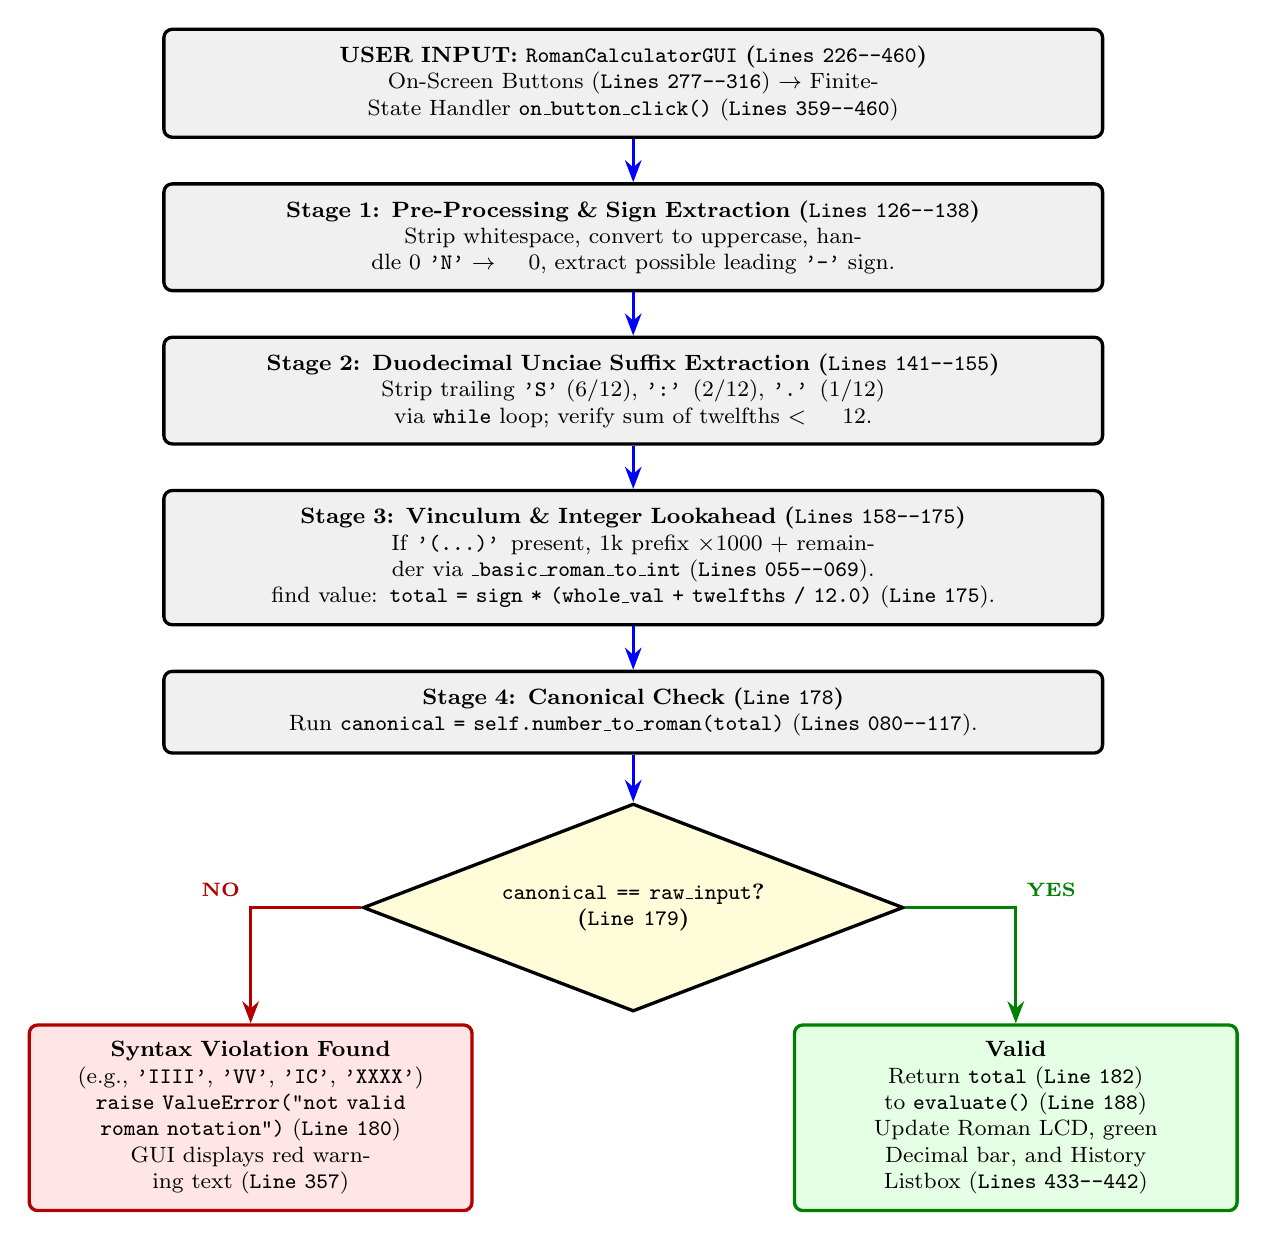
\begin{tikzpicture}[
    node distance=0.55cm and 1.2cm,
    box/.style={rectangle, rounded corners=3pt, draw=black, fill=black!6, very thick, text width=11.5cm, align=center, inner sep=6pt, font=\footnotesize},
    decision/.style={diamond, aspect=2.6, draw=black, fill=yellow!15, very thick, text width=4.8cm, align=center, inner sep=2pt, font=\footnotesize\bfseries},
    outcome_ok/.style={rectangle, rounded corners=3pt, draw=green!50!black, fill=green!10, very thick, text width=5.2cm, align=center, inner sep=6pt, font=\footnotesize},
    outcome_err/.style={rectangle, rounded corners=3pt, draw=red!70!black, fill=red!10, very thick, text width=5.2cm, align=center, inner sep=6pt, font=\footnotesize},
    arrow/.style={-{Stealth[length=2.8mm]}, very thick, color=blue}
]

\node[box] (gui) {
    \textbf{USER INPUT: \texttt{RomanCalculatorGUI} (\texttt{Lines 226--460})}\\
    On-Screen Buttons (\texttt{Lines 277--316}) $\rightarrow$ Finite-State Handler \texttt{on\_button\_click()} (\texttt{Lines 359--460})
};

\node[box, below=of gui] (step1) {
    \textbf{Stage 1: Pre-Processing \& Sign Extraction (\texttt{Lines 126--138})}\\
    Strip whitespace, convert to uppercase, handle 0 \texttt{'N'} $\rightarrow 0$, extract possible leading \texttt{'-'} sign.
};

\node[box, below=of step1] (step2) {
    \textbf{Stage 2: Duodecimal Unciae Suffix Extraction (\texttt{Lines 141--155}) }\\
    Strip trailing \texttt{'S'} ($6/12$), \texttt{':'} ($2/12$), \texttt{'.'} ($1/12$) via \texttt{while} loop; verify sum of twelfths $< 12$.
};

\node[box, below=of step2] (step3) {
    \textbf{Stage 3: Vinculum \& Integer Lookahead (\texttt{Lines 158--175}) }\\
    If \texttt{'(...)'} present, 1k prefix $\times 1000$ + remainder via \texttt{\_basic\_roman\_to\_int} (\texttt{Lines 055--069}).\\
    find value: \texttt{total = sign * (whole\_val + twelfths / 12.0)} (\texttt{Line 175}).
};

\node[box, below=of step3] (step4) {
    \textbf{Stage 4: Canonical Check (\texttt{Line 178}) }\\
    Run \texttt{canonical = self.number\_to\_roman(total)} (\texttt{Lines 080--117}).
};

\node[decision, below=0.6cm of step4] (check) {
    \texttt{canonical == raw\_input}?\\(\texttt{Line 179})
};

\node[outcome_err, below left=0.8cm and 0.3cm of check] (err) {
    \textbf{Syntax Violation Found}\\
    (e.g., \texttt{'IIII'}, \texttt{'VV'}, \texttt{'IC'}, \texttt{'XXXX'})\\
    \texttt{raise ValueError("not valid roman notation")} (\texttt{Line 180})\\
    GUI displays red warning text (\texttt{Line 357})
};

\node[outcome_ok, below right=0.8cm and 0.3cm of check] (ok) {
    \textbf{Valid }\\
    Return \texttt{total} (\texttt{Line 182}) to \texttt{evaluate()} (\texttt{Line 188})\\
    Update Roman LCD, green Decimal bar, and History Listbox (\texttt{Lines 433--442})
};

\draw[arrow] (gui) -- node[right, font=\scriptsize\itshape] {} (step1);
\draw[arrow] (step1) -- (step2);
\draw[arrow] (step2) -- (step3);
\draw[arrow] (step3) -- (step4);
\draw[arrow] (step4) -- (check);
\draw[arrow, color=red!70!black] (check.west) -| node[above left, font=\scriptsize\bfseries] {NO} (err.north);
\draw[arrow, color=green!50!black] (check.east) -| node[above right, font=\scriptsize\bfseries] {YES} (ok.north);

\end{tikzpicture}
\caption{Execution flow of the Calculator, highlighting the decoupling of the \texttt{tkinter} GUI state machine from the validation engine.}
\label{fig:flowchart}
\end{figure}

\section{Annotated Screenshots}

Figures \ref{fig:gui_ready} and \ref{fig:gui_calc} illustrate the operational \texttt{tkinter} desktop interface (\texttt{RomanCalculatorGUI}, \texttt{Lines 226--460}) in its initial ready state and during compound duodecimal fraction division.

\begin{figure}[h!]
    \centering
    \begin{subfigure}[t]{0.47\textwidth}
        \centering
        \safeimage[0.88\textwidth]{gui_ready.png}{GUI Screenshot 1: Ready State (N / Decimal: 0)}
        \caption{\textbf{Initial State} Upon launch (\texttt{Lines 247--269}), the calculator initialises to Nulla which acts as 0. The keypad (\texttt{Lines 277--316}) groups controls by function using TI-84/TI-89 high-contrast ergonomics: red clear/delete keys (\texttt{\#b71c1c}), charcoal Vinculum/sign/zero keys (\texttt{\#455a64}), white numeral keys (\texttt{\#f0f0f0}), grey operators/fractions (\texttt{\#8a8f99}), and a 3-column green calculate bar (\texttt{\#2e7d32}).}
        \label{fig:gui_ready}
    \end{subfigure}
    \hfill
    \begin{subfigure}[t]{0.47\textwidth}
        \centering
        \safeimage[0.88\textwidth]{gui_calc.png}{GUI Screenshot 2: Duodecimal Division (L:. / :. = CCI)}
        \caption{\textbf{Division:} Demonstrates exact compound duodecimal division (\texttt{Lines 422--445}) using the \textit{quadrans} ($\frac{3}{12}$, \texttt{:.}) notation documented in \cite{maher2001}: $50\frac{3}{12}$ (\texttt{L:.} $= 50.25$) divided by $\frac{3}{12}$ (\texttt{:.} $= 0.25$) yields \texttt{CCI} ($201$). The current expression (\texttt{L:. / :. =}), the main Roman result (\texttt{CCI}), the live decimal translation (\texttt{Decimal: 201}), and the Calculation History log update simultaneously.}
        \label{fig:gui_calc}
    \end{subfigure}
    \caption{Operational screenshots of the Calculator GUI.}
\end{figure}

\section{Complete Engine Verification \& Boundary-Test Matrix}

Table \ref{tab:fullmatrix} documents the systematic verification of \texttt{CalculatorMain.evaluate()} (\texttt{Lines 188--217}) and \texttt{CalculatorMain.roman\_to\_number()} (\texttt{Lines 121--182}) across classical literary test cases \cite{maher2001}, standard $1$--$3,999$ conversion benchmarks \cite{geeksforgeeks2021, steins2022}, extended numeral domains \cite{lewis2019}, and invalid syntax traps.

\begin{table}[h!]
\centering
\caption{Systematic Verification Matrix for \texttt{CalculatorMain} (\texttt{Lines 014--217})}
\label{tab:fullmatrix}
\footnotesize
\begin{tabular}{@{}llll@{}}
\toprule
\textbf{Test ID} & \textbf{Input Expression / String} & \textbf{Engine Output (\texttt{Roman} / \texttt{Decimal})} & \textbf{Target Mechanism \& Reference Verified} \\ \midrule
\textbf{T01} & \texttt{XIV + XXVI} & \texttt{XL} (\texttt{40}) & Standard additive/subtractive synthesis (\texttt{Lines 071--078}) \cite{steins2022, lewis2019} \\
\textbf{T02} & \texttt{MCMXCIV + VI} & \texttt{MM} (\texttt{2000}) & Subtractive lookahead \& carry propagation \cite{geeksforgeeks2021, steins2022} \\
\textbf{T03} & \texttt{L - L} & \texttt{N} (\texttt{0}) & Zero identity (\textit{Nulla}) handling (\texttt{Lines 082--083}) \\
\textbf{T04} & \texttt{X - XXV} & \texttt{-XV} (\texttt{-15}) & Signed negative Roman domain (\texttt{Lines 085--086}) \\
\textbf{T05} & \texttt{C * L} & \texttt{(V)} (\texttt{5000}) & Automatic \textit{Vinculum} scaling above $3,999$ (\texttt{Lines 102--105}) \cite{lewis2019} \\
\textbf{T06} & \texttt{(V) + D} & \texttt{(V)D} (\texttt{5500}) & Deep parentheses / \textit{Vinculum} input parsing (\texttt{Lines 160--171}) \cite{lewis2019} \\
\textbf{T07} & \texttt{::. - .} / \texttt{::. + .} & \texttt{::} (\texttt{0.333}) / \texttt{S} (\texttt{0.5}) & Horace \textit{Ars Poetica} \textit{unciae} drills ($\frac{5}{12} \mp \frac{1}{12}$) \cite{maher2001} \\
\textbf{T08} & \texttt{V * IS:.} & \texttt{VIIIS:.} (\texttt{8.75}) & Frontinus \textit{De aquaeductu} area ($5 \times 1\frac{3}{4} = 8\frac{3}{4}$) \cite{maher2001} \\
\textbf{T09} & \texttt{L:. / :.} & \texttt{CCI} (\texttt{201}) & Exact compound \textit{unciae} division ($50.25 \div 0.25$) \cite{maher2001} \\
\textbf{T10} & \texttt{X / III} & \texttt{III::} (\texttt{3.333}) & Base-12 \textit{triens} quantization ($3\frac{4}{12}$, \texttt{Lines 092--095}) \cite{maher2001} \\
\textbf{T11} & \texttt{XII \^{} III} & \texttt{MDCCXXVIII} (\texttt{1728}) & Exponentiation (\texttt{\^{}}, \texttt{Lines 212--213}) \\
\textbf{T12} & \texttt{IIII}, \texttt{VV}, \texttt{IC}, \texttt{XXXX} & \texttt{ValueError: not valid roman notation} & Canonical Round-Trip Validation (\texttt{Lines 178--180}) \cite{lewis2019} \\ \bottomrule
\end{tabular}
\end{table}

\end{document}